\section{Development Model}
\label{sec:development}

To satisfy the mission statement of the Project, the SunPy community adopted an open development model.
This development model is widely used within the scientific Python community.
The \sunpypkg package is hosted on \github and uses \code{git}\footnote{\url{https://git-scm.com/}} as its distributed version control software.
The entire codebase is publicly available and anyone can suggest changes through pull requests.
Since the codebase is licensed under a permissive 2-clause BSD license\footnote{\url{https://opensource.org/licenses/BSD-2-Clause}}, anyone can redistribute, improve, repackage or use it in a closed environment as long as they credit the SunPy developers and redistribute the license.
In order to maintain high quality code, every contribution must satisfy the following requirements:
\begin{enumerate}
    \item Code and documentation must follow widely used style guides (PEP 8 and numpydoc).
    \item All new features must be accompanied with documentation.
    This includes code comments, formal documentation, and gallery examples.
    \item Test code must be provided with coverage reports.
    \item Finally, all code must be within scope and be reviewed and accepted by at least two members of the developer community before it is integrated into the codebase.
\end{enumerate}
These requirements are imposed on every pull request regardless of contributor.

As of version 1.0, the \sunpypkg consists of 48,427 lines of code\footnote{This number includes documentation and comments. There are 30,906 lines of pure code.} contributed by 123 unique contributors over 11,659 \git commits. Figure~\ref{fig:metafig}, left, shows the steady growth of the code base since 2011 with, on average, approximately 16 lines added per day.
A reduction in the code base occurred after the release of version 0.9 due to a major clean up effort which led to the deletion of unused code and the removal of support for Python 2.

Figure~\ref{fig:metafig}, middle, shows the steady rise in the number of unique contributors with, on average, more than 1 new contributor added each month.

Figure~\ref{fig:metafig}, left, shows the distribution of total number of commits per contributor as of June 2019.
The distribution is relatively steep with a log-log slope of $-0.34$.
This means that relatively few authors generate the majority of commits.
The top 10 contributors are responsible for close to 80\% of the all commits. 

This compares poorly to other projects such as \astropy which have a flatter distribution (slope of $-0.5) \citep{astropy2018}.
Unlike \astropy, the \sunpyproj was not formed to bring together and coordinate many existing developers and their \python packages.
The development of the \sunpypkg package was begun with no prior existing code base by a core group of scientists.
It should be noted that the number of commits is only approximately related contribution size since a single commit could summarize a substantial increase in functionality or be a simple typographical fix.
Regardless, this distribution suggests that the core developer team has not grown substantially from that original core team.
On the other hand, the total number of unique commits is large which means that there exists a pool of \sunpypkg developers that are willing and have the knowledge to contribute.
We will need to put more effort into converting these contributors into core developers to improve the long-term health of the community.


\begin{figure}
    \center
    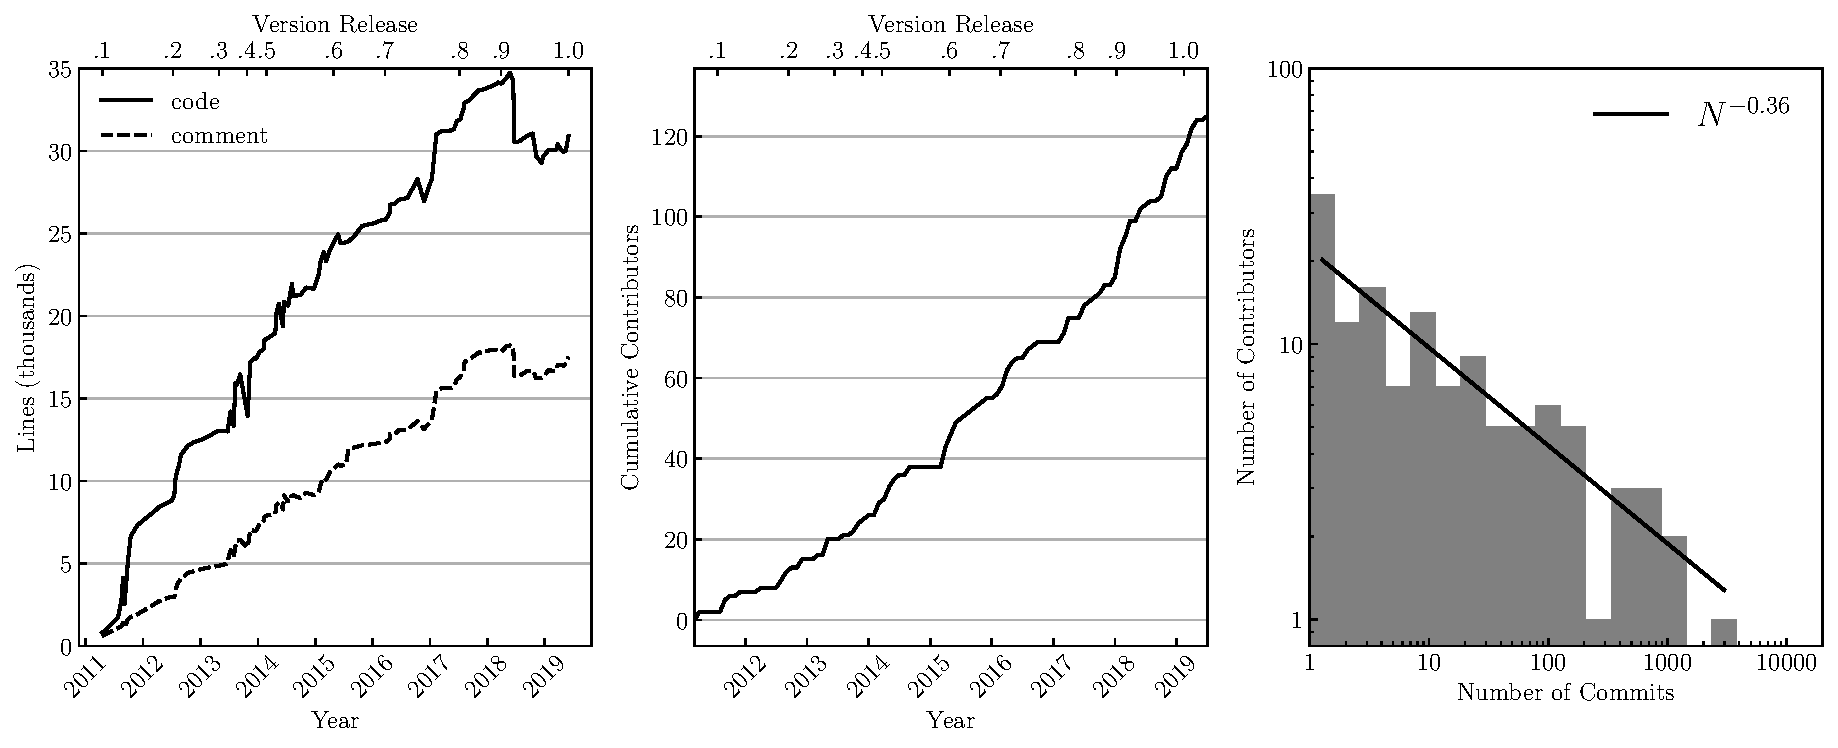
\includegraphics[width = 1.0\textwidth]{figures/dev_meta.pdf}
    \caption{Left panel: A plot of the steady increase in the total number of lines of code (solid line) and documentation line count (dotted line) as a function of time.
	Major releases are indicated.
	A striking reduction in the code base occurred after version 0.9.
	This period saw a major code organization and deletion of obsolete features along with removing support for Python 2.
	Middle panel: The cumulative number of committers (i.e. authors) to \sunpypkg as a function of time shows a steady increase in the number of people involved in the development team.
	Right panel: A plot of the distribution of the number of commits per commiter.
	Though commits is not the best measure this plot does indicates that the majority of commits are undertaken by the least amount of people with an average individual contribution of less than 10 commits.}
\label{fig:metafig}
\end{figure}